\documentclass[12pt,a4paper,oneside]{report}
\usepackage[margin=1in]{geometry}
\usepackage[T1]{fontenc}
\usepackage{lmodern,graphicx,booktabs,tabularx,array,longtable,multirow,float,amsmath,enumitem,tikz,caption,subcaption,placeins}
\usetikzlibrary{arrows.meta,positioning,shapes.geometric}
\usepackage[numbers,sort&compress]{natbib}
\usepackage[hidelinks]{hyperref}
\setlength{\parskip}{0.35em}\setlength{\parindent}{1.4em}\renewcommand{\arraystretch}{1.17}
\newcolumntype{Y}{>{\raggedright\arraybackslash}X}
\captionsetup{font=small,labelfont=bf}
\begin{document}
\begin{titlepage}\centering
{\large UNIVERSITY OF MUMBAI\par}\vspace{1.1cm}
{\Huge\bfseries AgriPredict\par}\vspace{0.3cm}
{\Large Multi-Crop Disease Classification and Agricultural Assistance System\par}\vspace{0.9cm}
{\large Project Report\par}\vspace{0.7cm}
Submitted in partial fulfillment of the requirements for the degree of\\
Bachelor of Technology in Electronics and Telecommunication Engineering\\[0.8cm]
Submitted by\\[0.2cm]
\rule{8cm}{0.3pt}\\[0.25cm]\rule{8cm}{0.3pt}\\[0.25cm]\rule{8cm}{0.3pt}\\[0.25cm]\rule{8cm}{0.3pt}\\[0.75cm]
Under the Guidance of\\\rule{8cm}{0.3pt}\\[0.9cm]
Department of Electronics and Telecommunication Engineering\\
Vidyalankar Institute of Technology, Mumbai\\Academic Year 2026--2027
\end{titlepage}
\pagenumbering{roman}
\chapter*{Abstract}\addcontentsline{toc}{chapter}{Abstract}
AgriPredict is a web-based agricultural support system combining crop-specific leaf-image classifiers with image checks, reliability-aware output, disease information, weather context, and a conversational agriculture assistant. The experiments cover nine crop models: Apple, Maize, Grapes, Tea, Potato, Cotton, Sugarcane, Groundnut, and Okra. The application crop selector lists eight crops; Groundnut is included here as a notebook-trained model and is not presented as enabled application support. The model implementations use ResNet50 features with crop-specific Transformer, multi-scale attention, spatial attention, or tile-view components. Recorded internal-test accuracy ranges from 88.86\% for Potato to 97.74\% for Maize. Selected crop workflows also apply confidence and embedding-neighbour rules to mark out-of-distribution inputs uncertain. This report follows the chapter organization in the University of Mumbai B.E. project-report guide and uses IEEE numbered citations and references.

\noindent\textbf{Keywords:} crop disease classification, ResNet50, Transformer, attention, image deduplication, out-of-distribution detection, agricultural assistant.
\tableofcontents\listoffigures\listoftables
\chapter*{Abbreviations and Acronyms}\addcontentsline{toc}{chapter}{Abbreviations and Acronyms}
\begin{longtable}{ll}CNN & Convolutional Neural Network\\OOD & Out-of-Distribution\\RAG & Retrieval-Augmented Generation\\ViT & Vision Transformer\\MLN & Maize Lethal Necrosis\\MSV & Maize Streak Virus\\NLB & Northern Leaf Blight\\NLS & Northern Leaf Streak\\pHash & Perceptual hash\\AUROC & Area Under the ROC Curve\\kNN & k-Nearest Neighbours\end{longtable}
\clearpage\pagenumbering{arabic}

\chapter{Introduction}
\section{Introduction}
Plant diseases and pest damage can reduce crop yield and quality. Image classification can support recognition of visible symptoms, but results depend on the crop and class labels represented during training, along with image quality and acquisition conditions. Previous work demonstrates the feasibility of deep learning for plant-leaf classification [\cite{hughes2015,mohanty2016}].

AgriPredict combines crop-specific image classification with input-quality checks and reliability decisions. It also provides disease information, weather context, and a farmer-oriented chat assistant. Image inference, weather retrieval, and conversational responses are separate application functions.
\section{Project Context and Motivation}
A classifier may return a label for an unclear or out-of-scope image. AgriPredict checks image quality before inference and, for selected crop models, applies a rejection policy that can mark an input uncertain. This report distinguishes crop models evaluated in notebooks from crops currently offered in the application.
\section{Aim and Contributions}
The aim is to develop and evaluate crop-specific leaf-image models and integrate them into an agricultural web application. The work records cleaned datasets and splits, implements ResNet50 hybrid architectures, evaluates classification and selected OOD outcomes, and integrates frontend, backend, disease information, weather context, and an agricultural assistant.
\section{Report Organization}
Chapter 2 presents related work, problem statement, objectives, and scope. Chapter 3 describes datasets and methodology. Chapter 4 describes implementation. Chapter 5 reports results. Chapter 6 concludes the report and identifies future scope.

\chapter{Literature Review}
\section{Literature Survey}
Residual connections support the optimization of deep convolutional networks [\cite{he2016}]. Vision Transformers use self-attention over image tokens [\cite{dosovitskiy2021}]. AgriPredict combines convolutional feature extraction with crop-specific Transformer or attention heads; the models are project implementations and are not exact reproductions of the supplied ResNet50+ViT papers.

PlantDoc provides field-style plant images that broaden evaluation beyond controlled leaf images [\cite{singh2020}]. Exact cryptographic hashes identify identical files; perceptual hashes identify visually similar candidates for review. Duplicate review helps reduce split leakage, while pHash candidates require visual confirmation [\cite{mckeown2023}].
\section{Problem Statement}
The project addresses how to build crop-specific leaf-image classifiers and present their outputs through a farmer-facing application while detecting unsuitable images and reducing unsupported predictions for inputs outside the trained class distribution.
\section{Objectives}
\begin{enumerate}[leftmargin=*]
\item Prepare crop datasets, class labels, and train, validation, and internal-test partitions.
\item Train crop-specific classifiers and select checkpoints using validation data.
\item Evaluate models using accuracy, balanced accuracy, macro-F1, and confusion matrices where available.
\item Evaluate confidence and embedding-neighbour rejection in crop workflows with OOD experiments.
\item Integrate supported models, image checks, guidance, weather context, and the farmer assistant in AgriPredict.
\end{enumerate}
\section{Scope of Project}
The model experiments document Apple, Maize, Grapes, Tea, Potato, Cotton, Sugarcane, Groundnut, and Okra. The application crop selector includes Apple, Maize, Grapes, Tea, Potato, Cotton, Sugarcane, and Okra [\cite{agripredict}]. Groundnut is included as a notebook-trained model and is not represented as live application support. Pear and Pumpkin are outside this report.

\chapter{Methodology}
\section{Datasets and Partitions}
Table~\ref{tab:splits} summarizes the cleaned project data. Source archive counts can differ from these working-set counts. Groundnut's original source describes six classes; the project classifier uses the five labels listed in Table~\ref{tab:classes}. The primary Portuguese grape data form the indicated split, with 358 additional field images used separately.
\begin{table}[H]\centering\small\caption{Cleaned dataset counts and partitions}\label{tab:splits}
\begin{tabularx}{\textwidth}{lrrrrY}\toprule Crop & Total & Train & Validation & Internal test & Dataset record\\\midrule
Apple&16,752&11,731&2,511&2,510&AppleLeaf9 + Indigenous Apple [\cite{appleleaf9,yatoo2024}]\\
Maize&8,239&5,762&1,239&1,238&Tanzania + CD\&S [\cite{mduma2025,ahmad2021}]\\
Grapes&5,255&3,678&788&789&Portuguese grape leaf RGB dataset [\cite{portela2026}]\\
Tea&1,681&1,176&252&253&Tea garden disease dataset [\cite{chowdhury2025}]\\
Potato&2,870&2,008&431&431&Six-class cleaned subset [\cite{shabrina2024}]\\
Cotton&1,648&1,149&249&250&Cleaned SAR-CLD-2024 subset [\cite{bishshash2024}]\\
Sugarcane&2,240&1,568&336&336&Cleaned sugarcane leaf disease set [\cite{daphal2024}]\\
Groundnut&3,036&2,125&455&456&Cleaned project subset [\cite{aishwarya2023}]\\
Okra&2,799&1,959&420&420&Five-class project subset [\cite{okra_dataset}]\\\bottomrule\end{tabularx}
\end{table}
The source record and the cleaned project count are different quantities. The Tea dataset record contains 2,500 naturally captured images from tea gardens in Habiganj, Sylhet, Bangladesh; the project used 1,681 after cleaning [\cite{chowdhury2025}]. The Potato source contains 3,076 images across seven labels; Nematode was excluded and the project used 2,870 images across six classes [\cite{shabrina2024}]. The Sugarcane archive contained 2,521 images before cleaning to 2,240 [\cite{daphal2024}]. The Groundnut publication describes 10,361 images across six source categories; the project model uses 3,036 images and five classes [\cite{aishwarya2023}]. The cotton paper describes 2,137 source images, while the project uses a cleaned 1,648-image subset [\cite{bishshash2024}]. The grape Zenodo record contains 5,267 original images; the cleaned Portuguese split uses 5,255, with 358 additional field images in a separate workflow [\cite{portela2026}]. The Okra archive used by the project contained 4,362 images before cleaning to 2,799; the Mendeley record with the matching class labels lists 4,267 images [\cite{okra_dataset}].
\begin{table}[H]\centering\small\caption{Class labels and available cleaned class counts}\label{tab:classes}\begin{tabularx}{\textwidth}{lY}\toprule Crop & Class labels and counts\\\midrule
Apple&Alternaria Leaf Spot; Brown Spot; Frogeye Leaf Spot; Mosaic; Powdery Mildew; Rust; Scab; Healthy Apple Leaf.\\
Maize&Healthy 2,376; MLN 2,388; MSV 2,443; NLB 489; NLS 543; GLS excluded.\\
Grapes&healthy; downy\_mildew; powdery\_mildew; esca\_complex; erineum\_mite.\\
Tea&Blight; Healthy Leaf; Helopeltis; Red Rust.\\
Potato&Bacteria 550; Fungi 716; Healthy 197; Pest 589; Phytopthora 300; Virus 518; Nematode excluded.\\
Cotton&Bacterial Blight; Curl Virus; Healthy Leaf; Leaf Hopper Jassids; Leaf Redding.\\
Sugarcane&Healthy 463; Mosaic 370; RedRot 491; Rust 440; Yellow 476.\\
Groundnut&early\_leaf\_spot; healthy leaf; late leaf spot; nutrition deficiency; rust.\\
Okra&Healthy\_Leaf 693; Insects\_Eaten\_Leaf 575; Leaf\_Curl 343; Leaf\_Spot 302; Yellow\_Vein\_Mosaic\_Virus 886; Fruit\_Rot excluded.\\\bottomrule\end{tabularx}\end{table}
Apple class counts are represented by the class-wise evaluation report in Section 5.2; other rows show class counts where recorded in the project dataset notes.
\section{Preprocessing and Duplicate Review}
The general procedure checked class-folder consistency and image readability, screened exact duplicates with SHA-256, and generated near-duplicate candidates with pHash. Candidate pairs were reviewed before removal or grouping because similar-looking leaves may be distinct samples. The thresholds and checks were crop-specific, as summarized in Table~\ref{tab:dedup}. Confirmed duplicates were removed or kept within one partition. Maize used a group-aware stratified split with seed 42 and had zero SHA-256 overlap across partitions. The sugarcane notebook flags 17 reviewed near-duplicate pairs crossing partitions.
\begin{table}[H]\centering\scriptsize\caption{Recorded crop-specific duplicate and split checks}\label{tab:dedup}\begin{tabularx}{\textwidth}{lY}\toprule Crop & Notebook-recorded checks\\\midrule
Apple&pHash hash size 8, Hamming distance $\leq10$ for candidate review across partitions; confirmed cross-split duplicates quarantined.\\
Maize&Group-aware stratified split, seed 42; zero exact SHA-256 overlap.\\
Grapes&SHA-256 and pHash distance 4 with visual review; 11 exact and 2 near duplicates removed from combined manifest.\\
Tea&SHA-256 and EXIF-orientation-robust pHash; distance 8 primary screen and broader candidate scan to 12; visual review and PlantDoc overlap check.\\
Potato&SHA-256, pHash distance 8, visual review, and tighter follow-up scan at distance 6.\\
Cotton&SHA-256 exact/label-conflict checks; pHash distance 8 candidates with review and group-aware partitioning.\\
Sugarcane&Exact duplicate checks and reviewed near-duplicate grouping; 17 cross-partition candidate pairs flagged.\\
Groundnut&Confirmed near-duplicate removal before split manifest.\\
Okra&Exact and reviewed near-duplicate removal before final split.\\\bottomrule\end{tabularx}\end{table}
\section{Crop-Specific Model Architectures}
The project uses more than one classifier design. Figure~\ref{fig:model} summarizes the architecture families; the per-crop layers are listed in Table~\ref{tab:architecture}. ResNet50 uses residual stages for visual feature extraction [\cite{he2016}].
\begin{figure}[H]\centering
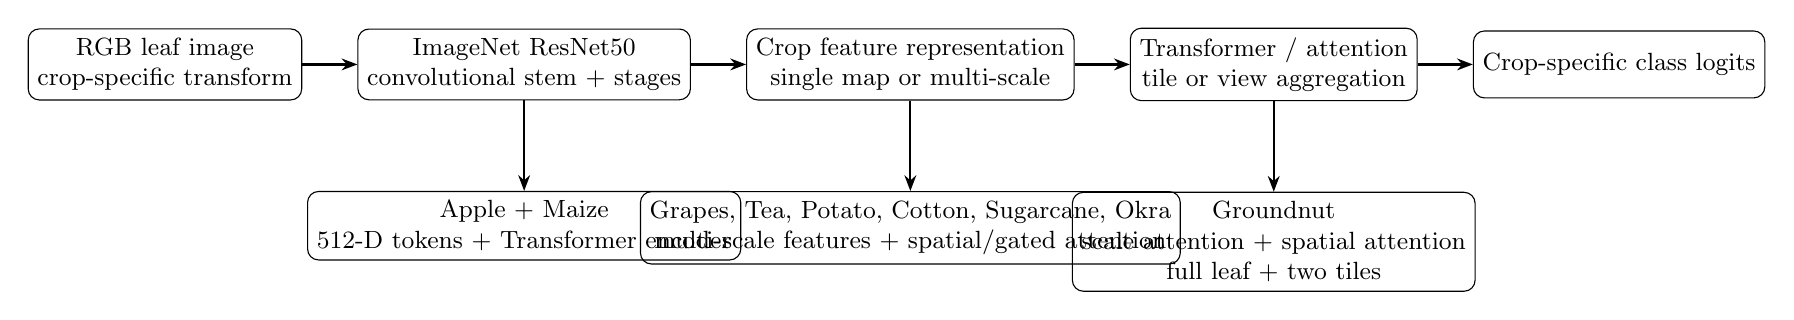
\begin{tikzpicture}[node distance=.55cm and .7cm,every node/.style={font=\small},b/.style={draw,rounded corners,align=center,minimum width=3.05cm,minimum height=.85cm},a/.style={-{Stealth[length=2mm]},thick}]
\node[b] (in) {RGB leaf image\\crop-specific transform};\node[b,right=of in] (res) {ImageNet ResNet50\\convolutional stem + stages};\node[b,right=of res] (feat) {Crop feature representation\\single map or multi-scale};\node[b,right=of feat] (head) {Transformer / attention\\tile or view aggregation};\node[b,right=of head] (cls) {Crop-specific class logits};\draw[a](in)--(res);\draw[a](res)--(feat);\draw[a](feat)--(head);\draw[a](head)--(cls);
\node[b,below=1.15cm of res,minimum width=4cm] (am) {Apple + Maize\\512-D tokens + Transformer encoder};\node[b,below=1.15cm of feat,minimum width=4.1cm] (multi) {Grapes, Tea, Potato, Cotton, Sugarcane, Okra\\multi-scale features + spatial/gated attention};\node[b,below=1.15cm of head,minimum width=3.7cm] (gn) {Groundnut\\scale attention + spatial attention\\full leaf + two tiles};
\draw[a](res.south)--(am.north);\draw[a](feat.south)--(multi.north);\draw[a](head.south)--(gn.north);
\end{tikzpicture}
\caption{Crop-specific model architecture families implemented in project notebooks.}\label{fig:model}\end{figure}
\begin{longtable}{p{1.2cm}p{13.5cm}}\caption{Crop model architecture details}\label{tab:architecture}\\\toprule Model & Implemented feature and classifier path\\\midrule\endfirsthead\toprule Model & Implemented feature and classifier path\\\midrule\endhead
Apple&ImageNet ResNet50 without average-pool and FC produces $B\times2048\times7\times7$. A $1\times1$ convolution projects 2048 to 512. The $7\times7$ grid becomes 49 learned-position tokens. Two Transformer encoder layers use 8 heads, 2048-dimensional FFN, GELU, pre-LayerNorm, and dropout 0.2. Mean token pooling, LayerNorm, dropout, and a linear 8-class classifier produce logits.\\
Maize&ResNet50 feature map projected $2048\to512$, 64 tokens for 256-pixel input, learned positions, and four Transformer encoder layers with 8 heads and FFN 2048. The head uses dropout, a 256-unit GELU layer, dropout, and five-class output.\\
Grapes&ResNet50 layers 2, 3, and 4 provide multi-scale features; projection/fusion and spatial self-attention encode image views, then full-image/tile views contribute to classification.\\
Tea&ResNet50 multi-scale features followed by gated spatial self-attention and full-image/tile inputs, pooling, and a four-class head.\\
Potato&ResNet50 multi-scale projection/fusion, gated spatial attention, and tile aggregation followed by the six-class head.\\
Cotton&ResNet50 layers 2/3/4 are projected and fused; spatial self-attention encodes each view. The full image and four tiles are combined by mean aggregation before classification.\\
Sugarcane&ResNet50 multi-scale feature fusion with spatial self-attention and full/tile aggregation, followed by the five-class head.\\
Groundnut&ResNet50 layer2/3/4 pooled features are projected to 256-D scale tokens and processed by 4-head scale attention. Layer4 is pooled to $7\times7$, projected to 256-D and processed by 4-head spatial attention. The two features concatenate, project to 512-D with GELU/dropout 0.30, then classify. Three views (full leaf and two overlapping tiles) are averaged.\\
Okra&ResNet50 layers 2/3/4 are projected to 256 channels and aligned to layer-2 resolution, concatenated, fused by a $3\times3$ convolution, and processed by gated 8-head spatial attention. Tile/view scores are aggregated before the five-class head.\\\bottomrule\end{longtable}
\subsection{Apple ResNet50--Transformer Layer Flow}
The Apple network takes a normalized RGB tensor through the ResNet50 stem and residual stages. The last convolutional output has 2048 channels over a $7\times7$ grid. A pointwise convolution reduces it to 512 channels. The 49 grid locations are flattened into 512-dimensional tokens and receive learned positional embeddings. Two pre-normalized Transformer encoder blocks perform eight-head self-attention and 2048-unit feed-forward transformations with GELU and dropout 0.2. Average pooling across tokens yields a 512-dimensional vector; LayerNorm and dropout precede the 8-class linear head. This 512-dimensional representation also feeds the Apple kNN reliability stage. The design is an implementation in the project notebook, not an exact copy of an external ResNet50--ViT paper.
\section{Training, Checkpoint Selection, and Metrics}
Each crop notebook defines its own input preprocessing, augmentation, class mapping, and training configuration. Checkpoints were selected using validation macro-F1 where recorded. The untouched internal-test partition is used for reported final classification metrics. Accuracy is correct predictions divided by all examples; balanced accuracy is mean class recall; macro-F1 is the unweighted average of class F1. Confusion matrices use true classes by row and predictions by column.
\section{Out-of-Distribution Decision}
Selected crop workflows compare classifier confidence and image embeddings against a crop-specific kNN reference. The calibrated threshold policy marks a sample ACCEPT or UNCERTAIN. PlantDoc is used as a held-out non-target image set in selected experiments [\cite{singh2020}]. AUROC, acceptance rate, rejection rate, and accepted-only accuracy measure different aspects and are reported separately.

\chapter{Implementation}
\section{Software Architecture}
Figure~\ref{fig:system} shows the application paths. The frontend is React/Vite and the backend is FastAPI. Crop selection routes the image to the corresponding model configuration and inference adapter. Image validation is performed before model inference. A reliability stage returns a prediction or an uncertain outcome. Disease information and weather context are presented separately. The Assistant chat runs through its own retrieval-and-generation path.
\begin{figure}[H]\centering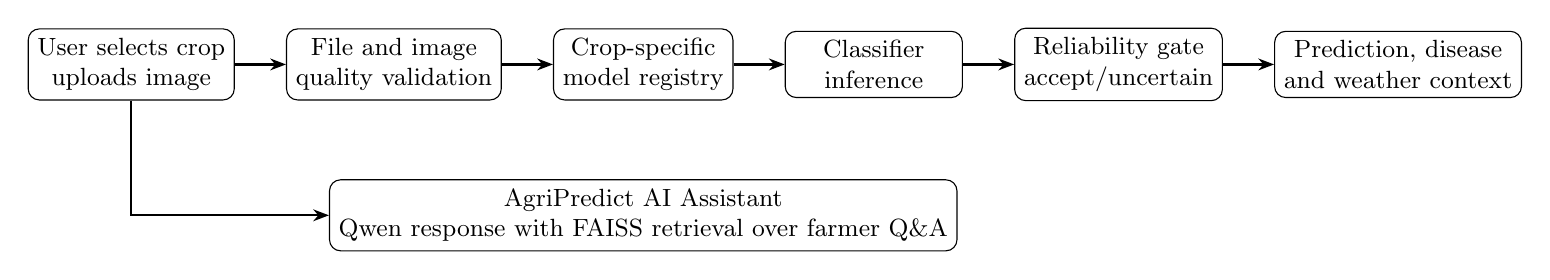
\begin{tikzpicture}[node distance=.65cm and .65cm,every node/.style={font=\small},b/.style={draw,rounded corners,align=center,minimum width=2.25cm,minimum height=.8cm},a/.style={-{Stealth[length=2mm]},thick}]
\node[b](ui){User selects crop\\uploads image};\node[b,right=of ui](val){File and image\\quality validation};\node[b,right=of val](reg){Crop-specific\\model registry};\node[b,right=of reg](inf){Classifier\\inference};\node[b,right=of inf](gate){Reliability gate\\accept/uncertain};\node[b,right=of gate](out){Prediction, disease\\and weather context};\draw[a](ui)--(val);\draw[a](val)--(reg);\draw[a](reg)--(inf);\draw[a](inf)--(gate);\draw[a](gate)--(out);
\node[b,below=1.0cm of reg,minimum width=5cm](chat){AgriPredict AI Assistant\\Qwen response with FAISS retrieval over farmer Q\&A};\draw[a](ui.south)|-(chat.west);
\end{tikzpicture}\caption{AgriPredict image-prediction path and separate assistant path.}\label{fig:system}\end{figure}
\section{Frontend and Backend}
The React/Vite frontend contains crop selection, image upload, prediction results, and the Agriculture Assistant chat interface. The FastAPI backend validates requests, dispatches the selected crop to its configured model adapter, runs inference, and returns a class prediction and reliability state. Image checks cover unreadable, blurry, poorly lit, overexposed, and low-resolution files. The application selector currently exposes eight crops; Groundnut is not in that selector.
\section{AgriPredict AI Assistant}
The assistant is independent of the image classifier. Its authenticated API accepts a question and conversation history. The configured service loads Qwen3-0.6B with a QLoRA adapter, embeds queries with all-MiniLM-L6-v2, retrieves up to five records from a FAISS index, and generates a response using the retrieved farmer-oriented question-and-answer corpus. A retrieval threshold of 0.60 is configured. The corpus stores question/response and agricultural, location, date, and language metadata. No corpus citation is assigned in this report because the supplied project materials do not identify its published source.
\section{Disease and Weather Services}
The app presents crop/class disease guidance and weather context in separate response components. Weather is retrieved after image inference and is not a classifier input. The assistant response is another distinct service output.

\chapter{Experimental Results}
\section{Aggregate Classification Results}
Table~\ref{tab:results} consolidates the crop evaluation document. Scores describe the recorded project internal partitions.
\begin{table}[H]\centering\small\caption{Validation and internal-test classification scores}\label{tab:results}\begin{tabularx}{\textwidth}{lrrrrrrr}\toprule Crop & Val. acc. & Val. bal. acc. & Val. macro-F1 & Test acc. & Test bal. acc. & Test macro-F1 & Test $n$\\\midrule
Apple&97.01\%&--&0.9722&96.22\%&--&0.9676&2510\\Maize&97.26\%&98.11\%&0.9810&97.74\%&98.45\%&0.9844&1238\\Grapes&--&--&--&96.58\%&96.61\%&0.9661&789\\Tea&94.84\%&95.06\%&0.9482&93.28\%&93.42\%&0.9319&253\\Potato&89.10\%&88.90\%&0.8791&88.86\%&88.96\%&0.8807&431\\Cotton&94.38\%&96.12\%&0.9435&92.80\%&94.35\%&0.9306&250\\Sugarcane&--&--&0.9833&97.62\%&97.76\%&0.9763&336\\Groundnut&92.09\%&93.82\%&0.9400&94.96\%&95.69\%&0.9611&456\\Okra&93.81\%&92.93\%&0.9257&95.71\%&95.61\%&0.9511&420\\\bottomrule\end{tabularx}\end{table}
The Sugarcane validation summary contains macro-F1 only. Apple validation and test balanced accuracy are not included in the supplied score summary. The Grape row reports the baseline Portuguese internal-test result; the field-adapted matrix below is a separate evaluation output.
\section{Apple Results and Confusion Matrices}
The Apple selected checkpoint achieved 97.01\% validation accuracy and 0.9722 validation macro-F1 on 2,511 images. On the 2,510-image internal test split, it achieved 96.22\% accuracy and 0.9676 macro-F1. Table~\ref{tab:appleclass} shows its internal-test class metrics.
\begin{table}[H]\centering\small\caption{Apple internal-test class metrics}\label{tab:appleclass}\begin{tabular}{lrrrr}\toprule Class & Precision & Recall & F1 & Support\\\midrule Alternaria Leaf Spot&0.9829&0.9787&0.9808&235\\Brown Spot&0.9821&1.0000&0.9910&55\\Frogeye Leaf Spot&0.9621&0.9581&0.9601&477\\Mosaic&0.9804&0.9950&0.9877&201\\Powdery Mildew&1.0000&0.9266&0.9619&177\\Rust&0.9619&0.9323&0.9469&325\\Scab&0.9543&0.9614&0.9579&804\\Healthy Apple Leaf&0.9246&0.9873&0.9549&236\\\bottomrule\end{tabular}\end{table}
\begin{figure}[H]\centering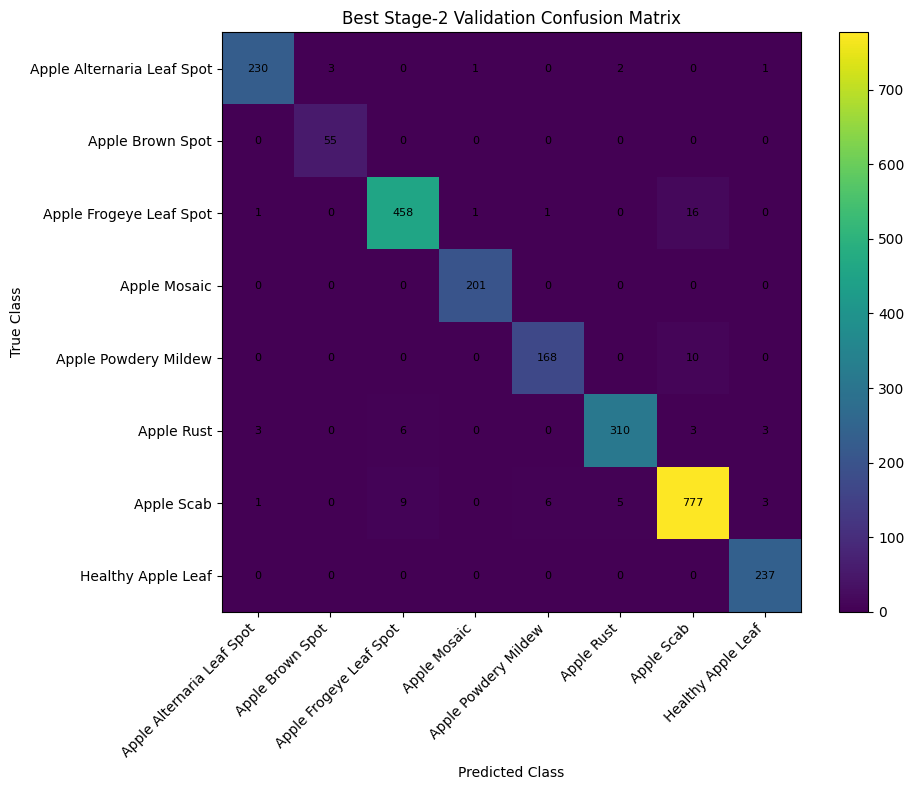
\includegraphics[width=.9\textwidth]{figures/apple_validation.png}\caption{Apple best Stage-2 validation confusion matrix.}\end{figure}
\begin{figure}[H]\centering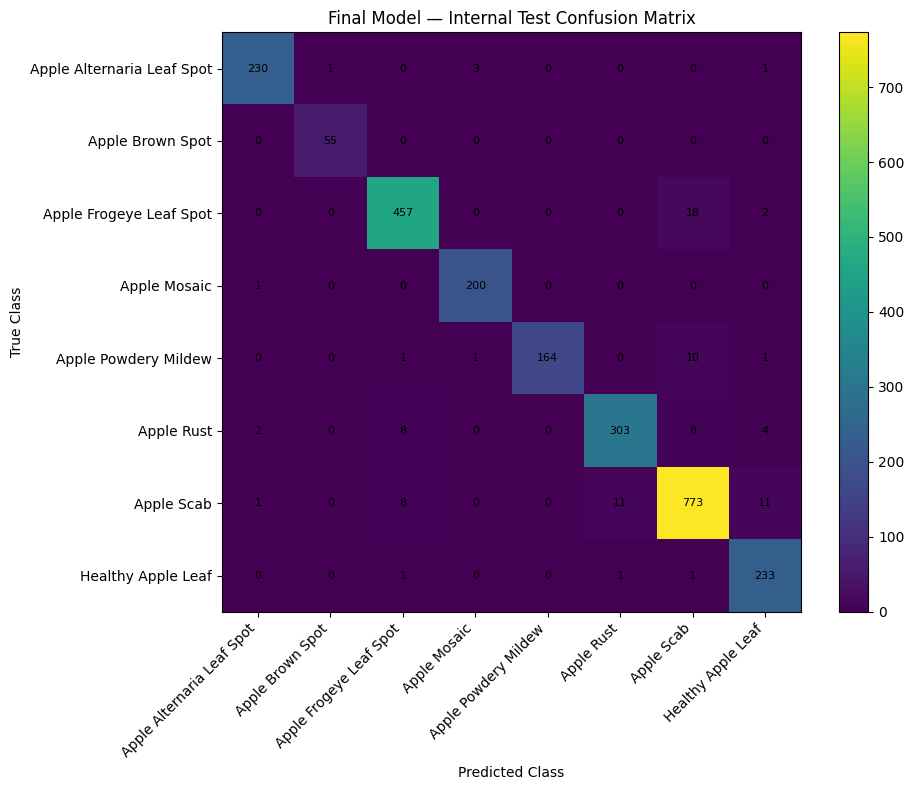
\includegraphics[width=.9\textwidth]{figures/apple_test.png}\caption{Apple final internal-test confusion matrix.}\end{figure}
\section{Maize and Grape Confusion Matrices}
Maize achieved 97.74\% test accuracy, 98.45\% balanced accuracy, and 0.9844 macro-F1 on 1,238 images. Figure~\ref{fig:maizeval} and Figure~\ref{fig:maizetest} show its supplied matrices.
\begin{figure}[H]\centering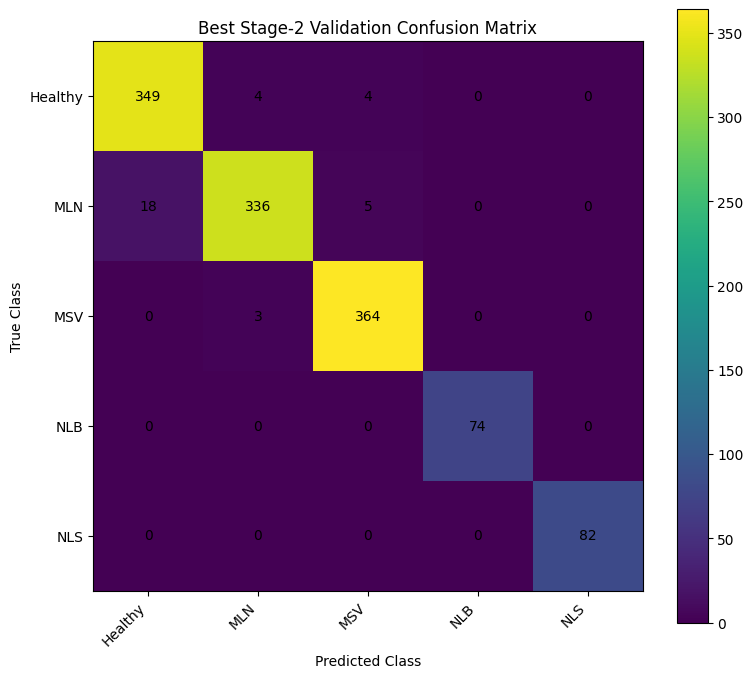
\includegraphics[width=.82\textwidth]{figures/maize_validation.png}\caption{Maize best Stage-2 validation confusion matrix.}\label{fig:maizeval}\end{figure}
\begin{figure}[H]\centering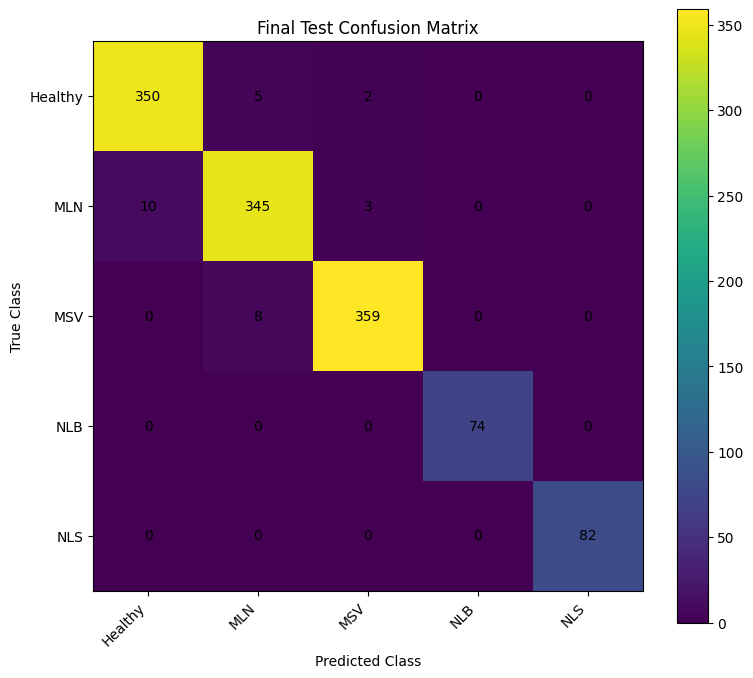
\includegraphics[width=.82\textwidth]{figures/maize_test.png}\caption{Maize final internal-test confusion matrix.}\label{fig:maizetest}\end{figure}
The baseline Grape model achieved 96.58\% accuracy and 0.9661 macro-F1 on 789 Portuguese test images. Figure~\ref{fig:grapetest} shows the separate field-adapted model matrix supplied for the Portuguese internal test.
\begin{figure}[H]\centering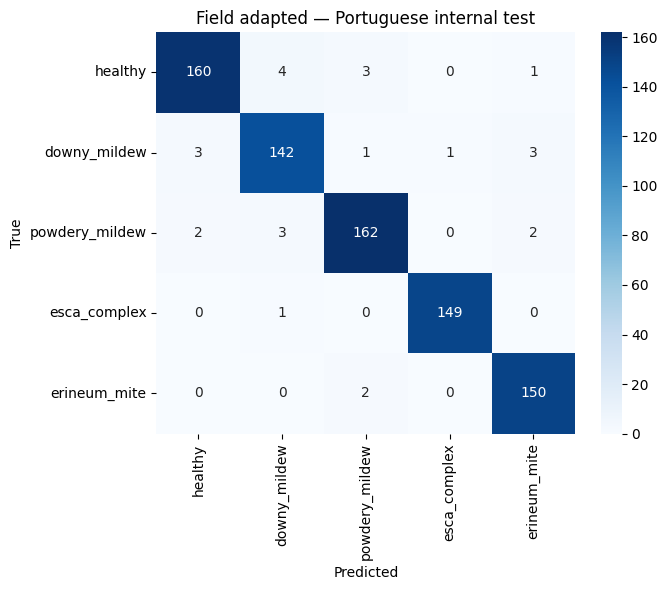
\includegraphics[width=.75\textwidth]{figures/grape_field_adapted.png}\caption{Field-adapted Grape model confusion matrix on the Portuguese internal-test set.}\label{fig:grapetest}\end{figure}
\section{Other Crop Confusion Matrices}
Each matrix has true classes by row and predicted classes by column. For space, these confusion matrices are typeset as tables.
\begin{table}[H]\centering\scriptsize\caption{Tea validation confusion matrix}\begin{tabular}{lrrrr}\toprule & Blight & Healthy & Helopeltis & Red Rust\\\midrule Blight&54&0&0&2\\Healthy&0&60&0&0\\Helopeltis&1&5&62&0\\Red Rust&4&1&0&63\\\bottomrule\end{tabular}\end{table}
\begin{table}[H]\centering\scriptsize\caption{Tea internal-test confusion matrix}\begin{tabular}{lrrrr}\toprule & Blight & Healthy & Helopeltis & Red Rust\\\midrule Blight&51&1&0&4\\Healthy&0&59&0&0\\Helopeltis&2&2&65&0\\Red Rust&4&3&1&61\\\bottomrule\end{tabular}\end{table}
\begin{table}[H]\centering\scriptsize\caption{Cotton internal-test confusion matrix}\begin{tabular}{lrrrrr}\toprule & Bacterial Blight & Curl Virus & Healthy & Jassids & Redding\\\midrule Bacterial Blight&38&0&0&0&0\\Curl Virus&0&64&0&1&0\\Healthy&0&0&27&0&0\\Jassids&1&3&0&31&0\\Redding&3&3&0&7&72\\\bottomrule\end{tabular}\end{table}
\begin{table}[H]\centering\scriptsize\caption{Sugarcane internal-test confusion matrix}\begin{tabular}{lrrrrr}\toprule & Healthy & Mosaic & RedRot & Rust & Yellow\\\midrule Healthy&69&0&0&0&0\\Mosaic&0&56&0&0&0\\RedRot&2&0&71&1&0\\Rust&0&0&0&65&1\\Yellow&0&2&0&2&67\\\bottomrule\end{tabular}\end{table}
\begin{table}[H]\centering\scriptsize\caption{Potato validation confusion matrix}\begin{tabular}{lrrrrrr}\toprule & Bacteria & Fungi & Healthy & Pest & Phytopthora & Virus\\\midrule Bacteria&79&1&0&2&0&0\\Fungi&0&98&2&6&1&1\\Healthy&0&0&27&1&0&1\\Pest&0&5&5&78&0&1\\Phytopthora&1&6&0&1&37&0\\Virus&1&2&7&2&1&65\\\bottomrule\end{tabular}\end{table}
\begin{table}[H]\centering\scriptsize\caption{Potato internal-test confusion matrix}\begin{tabular}{lrrrrrr}\toprule & Bacteria & Fungi & Healthy & Pest & Phytopthora & Virus\\\midrule Bacteria&77&3&0&3&0&0\\Fungi&1&99&0&4&3&0\\Healthy&0&0&30&0&0&0\\Pest&0&4&6&78&0&0\\Phytopthora&0&8&0&2&35&0\\Virus&2&4&6&2&0&64\\\bottomrule\end{tabular}\end{table}
\begin{table}[H]\centering\scriptsize\caption{Groundnut internal-test confusion matrix}\begin{tabular}{lrrrrr}\toprule & Early leaf spot & Healthy leaf & Late leaf spot & Nutrition deficiency & Rust\\\midrule Early leaf spot&118&14&0&0&0\\Healthy leaf&7&131&0&0&0\\Late leaf spot&0&0&103&0&0\\Nutrition deficiency&0&0&0&49&0\\Rust&1&0&1&0&32\\\bottomrule\end{tabular}\end{table}
\begin{table}[H]\centering\scriptsize\caption{Okra internal-test confusion matrix}\begin{tabular}{lrrrrr}\toprule & Healthy Leaf & Insects Eaten & Leaf Curl & Leaf Spot & Yellow Vein Mosaic\\\midrule Healthy Leaf&103&0&1&0&0\\Insects Eaten&5&76&1&4&0\\Leaf Curl&0&1&51&0&0\\Leaf Spot&0&1&1&43&0\\Yellow Vein Mosaic&1&2&1&0&129\\\bottomrule\end{tabular}\end{table}
\section{Out-of-Distribution Results}
Table~\ref{tab:ood} summarizes the frozen operating-point results. Apple is the only crop with AUROC recorded in the supplied evaluation.
\begin{table}[H]\centering\scriptsize\caption{Crop-specific OOD evaluation at the recorded thresholds}\label{tab:ood}\begin{tabularx}{\textwidth}{lYYYY}\toprule Crop & Calibration rule & In-distribution test & Held-out OOD test & Additional recorded result\\\midrule
Apple&kNN $K=10$, threshold 0.9357&95.30\% accepted (2,510)&83.09\% rejected (207 non-Apple PlantDoc)&AUROC 0.9631\\
Grapes&kNN 0.916923; confidence 0.594393&98.7\% accepted (789); accepted accuracy 97.0\%&99.5\% rejected (205 other-crop PlantDoc); 74.0\% (50 unsupported grape)&Black Rot 90\% rejected; Leaf Blight 70\% rejected\\
Tea&Confidence 0.2686 and kNN 0.8942, $K=10$&237/253 accepted (93.7\%); pre-rejection accuracy 90.91\%, macro-F1 0.9071&226/228 PlantDoc rejected (99.1\%)&Accepted accuracy 92.83\%; no AUROC\\
Cotton&Frozen confidence plus kNN policy&246/250 accepted; accepted accuracy 93.09\%&78/236 PlantDoc test rejected (33.05\%); validation rejection 91/271 (33.58\%)&A grape example passed as Leaf Redding\\
Sugarcane&Confidence 0.57815 and kNN 0.8175, $K=10$&325/336 accepted (96.7\%); pre-rejection accuracy 91.96\%, macro-F1 0.9182&204/228 PlantDoc rejected (89.5\%)&Accepted accuracy 93.85\%; no AUROC\\
Okra&Confidence 0.3917 and kNN 0.9663, $K=10$&414/420 accepted (98.6\%); pre-rejection accuracy 95.24\%, macro-F1 0.9431&227/228 PlantDoc rejected (99.6\%)&Accepted accuracy 95.89\%; no AUROC\\
Maize, Potato, Groundnut&--&--&--&No OOD evaluation result recorded\\\bottomrule\end{tabularx}\end{table}

\chapter{Conclusion and Future Scope}
\section{Conclusion}
AgriPredict combines crop-specific leaf-image classification with image-quality checks, reliability decisions, disease information, weather context, and a separate agricultural question-answer assistant. Nine crop model experiments are documented; the application selector exposes eight crops, and Groundnut is reported as a notebook-trained model rather than an enabled application crop. The model implementations use ResNet50 with crop-specific Transformer, multi-scale attention, spatial attention, or multi-view designs. Recorded internal-test accuracy ranges from 88.86\% for Potato to 97.74\% for Maize. OOD behavior varies across crop workflows and datasets and is reported at the tested thresholds.
\section{Future Scope}
Future work includes evaluating models on independent field images across farms, seasons, devices, and symptom stages; extending the application to additional notebook models after verifying packaging and class mappings; repeating OOD evaluation for all application crops; measuring inference latency and application usability; reviewing the sugarcane cross-partition near-duplicate flags; and evaluating assistant retrieval and answer quality with agricultural experts.

\bibliographystyle{IEEEtran}\bibliography{references}
\end{document}
